

\documentclass[a4paper]{article}

\usepackage{amsmath}
\usepackage{hyperref}
\usepackage{biblatex}
\usepackage{enumerate}
\usepackage{graphicx}
\usepackage{stmaryrd}
\usepackage[dvipsnames]{xcolor}
\usepackage{listings}
\usepackage{caption}
\usepackage{subcaption}
\usepackage{booktabs}


\addbibresource{refs.bib}

\begin{document}

\author{Ola Bratt \\
  \href{mailto:ola.bratt@gmail.com}{ola.bratt@gmail.com}
  \and
  Patrick Attimont \\
  \href{patrickattimont@gmail.com}{patrickattimont@gmail.com}
}

\title{DAT565/DIT407 Assignment 4}
\date{2024-02-xx}

\maketitle

This paper is addressing the assignment 3 study queries within the \emph{Introduction to Data Science \& AI} course, DIT407 at 
the University of Gothenburg and DAT565 at Chalmers. The main source of information for this project
is derived from the lectures and Skiena~\cite{Skiena:2024}. Assignment 4 is about correlation and linear regression.

\section*{Problem 1: Splitting the data}



\section*{Problem 2: Single-variable model}
The variable 'Human Development Index (value)' has the strongest pearson correlation with a coefficient of 0.92.
Trained model with the following variables :  Human Development Index (value)
The mean squared error for is 9.45.


\begin{figure}[h]
  \begin{center}
    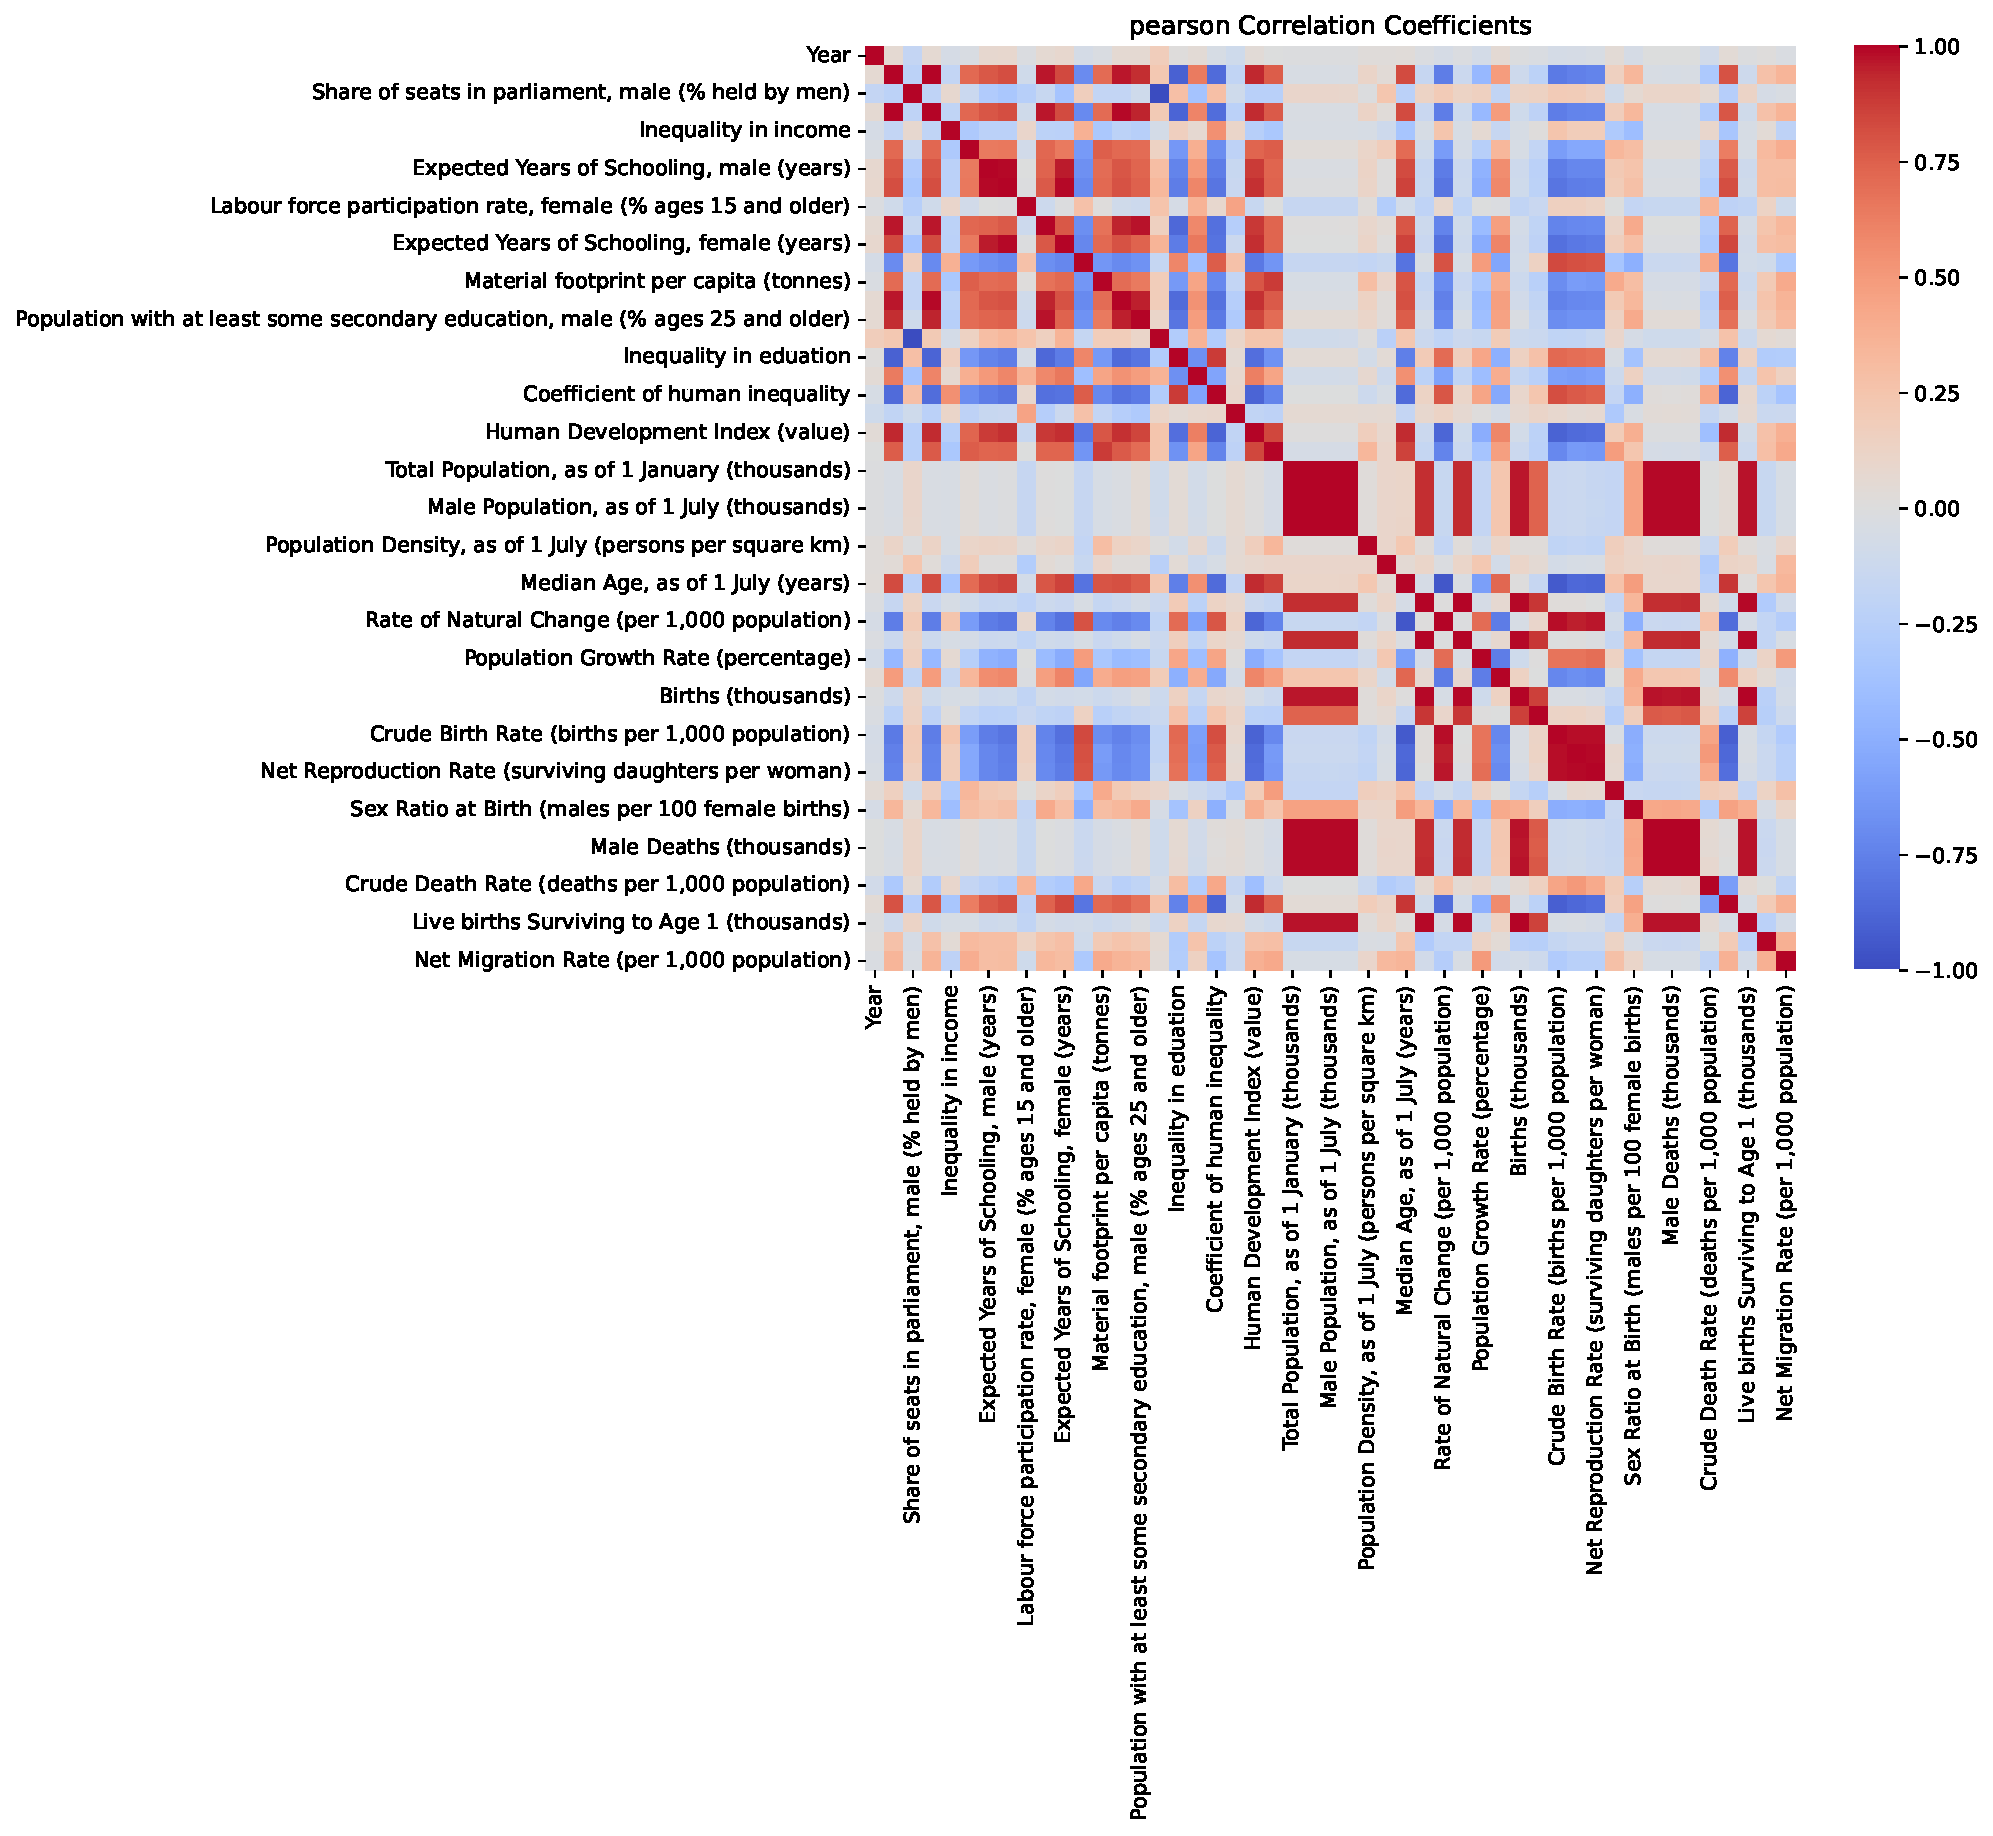
\includegraphics[width=\textwidth]{ola/pearson_correlation.pdf}
    \caption{Correlation Pearson}
    \label{fig:pearson_correlation}
  \end{center}
\end{figure}

\begin{figure}[h]
  \begin{center}
    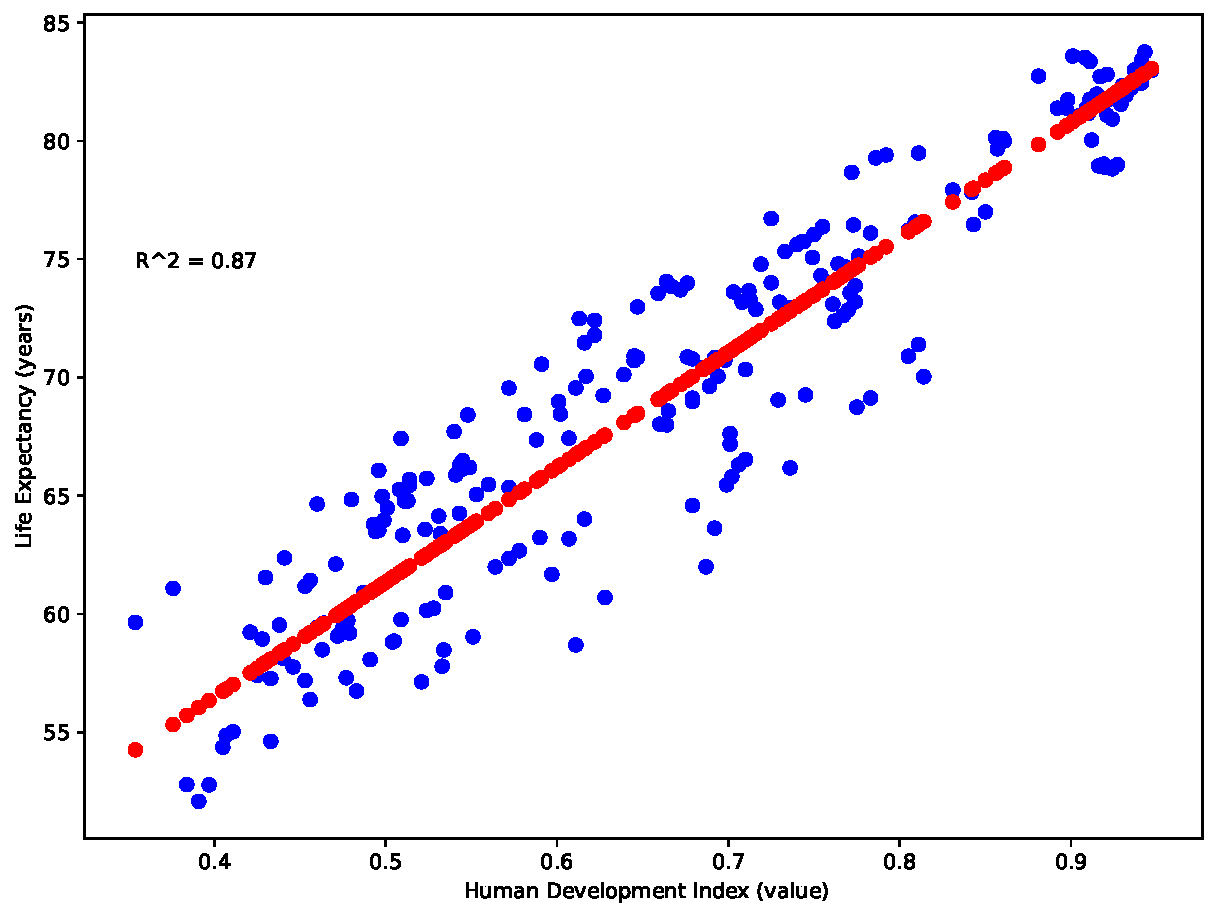
\includegraphics[width=\textwidth]{ola/_linear_regression_human_development_index_(value).pdf}
    \caption{Linear Regression Human Development Index (value)}
    \label{fig:reg_human_development_index}
  \end{center}
\end{figure}

\section*{Problem 3: Non-linear relationship}

The variable 'Median Age, as of 1 July (years)' has the strongest spearman correlation with a coefficient of 0.91.
Trained model with the following variables :  Median Age, as of 1 July (years)
The mean squared error for is 13.58.
Trained model with the following variables [Log]:  Median Age, as of 1 July (years)
The mean squared error for is 11.52.
Trained model with the following variables [Sqrt]:  Median Age, as of 1 July (years)
The mean squared error for is 12.23.
Trained model with the following variables [Reciprocal]:  Median Age, as of 1 July (years)
The mean squared error for is 12.12.

\begin{figure}[h]
  \begin{center}
    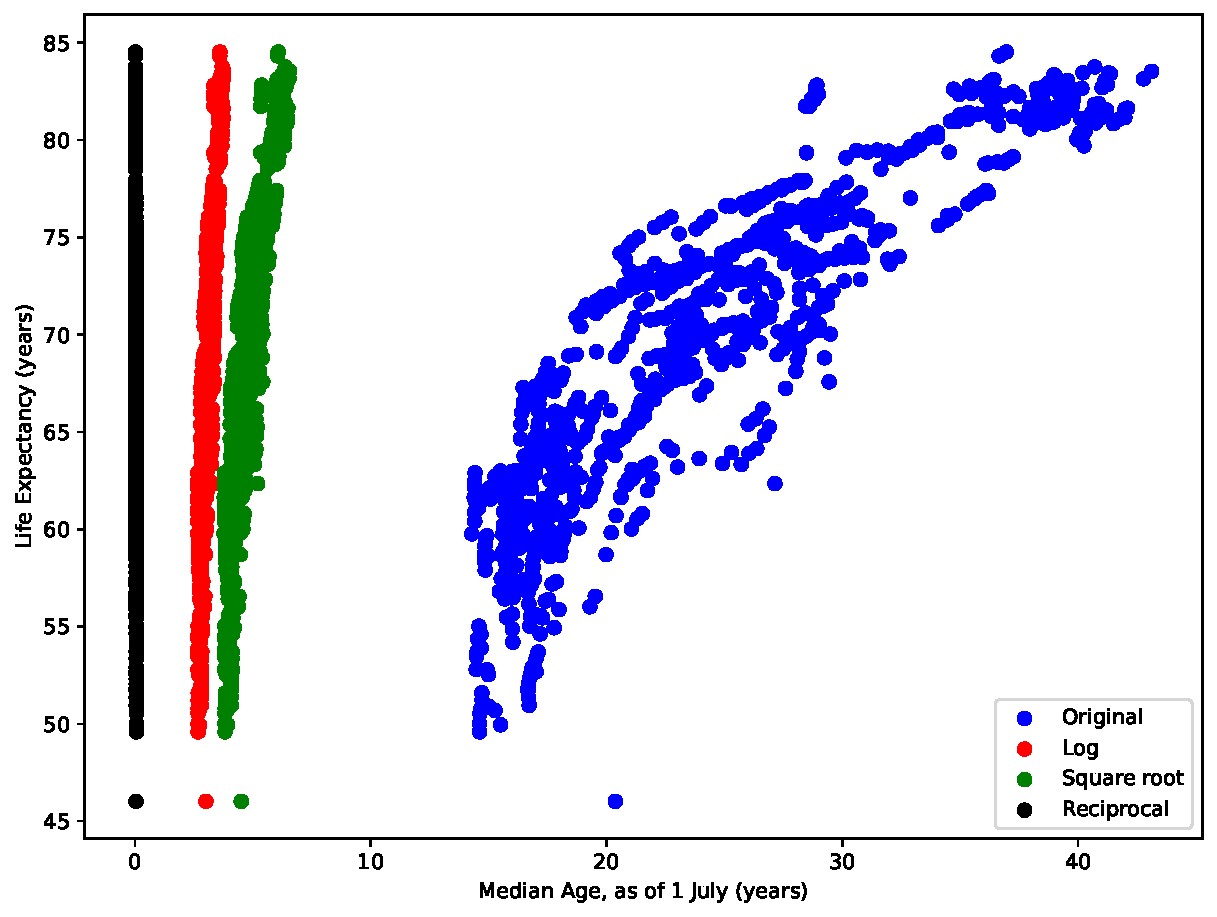
\includegraphics[width=\textwidth]{ola/linear_transformation.pdf}
    \caption{Linear transformation}
    \label{fig:linear_transformation}
  \end{center}
\end{figure}

\begin{figure}
  \centering
  \begin{subfigure}[a]{\textwidth}
      \centering
      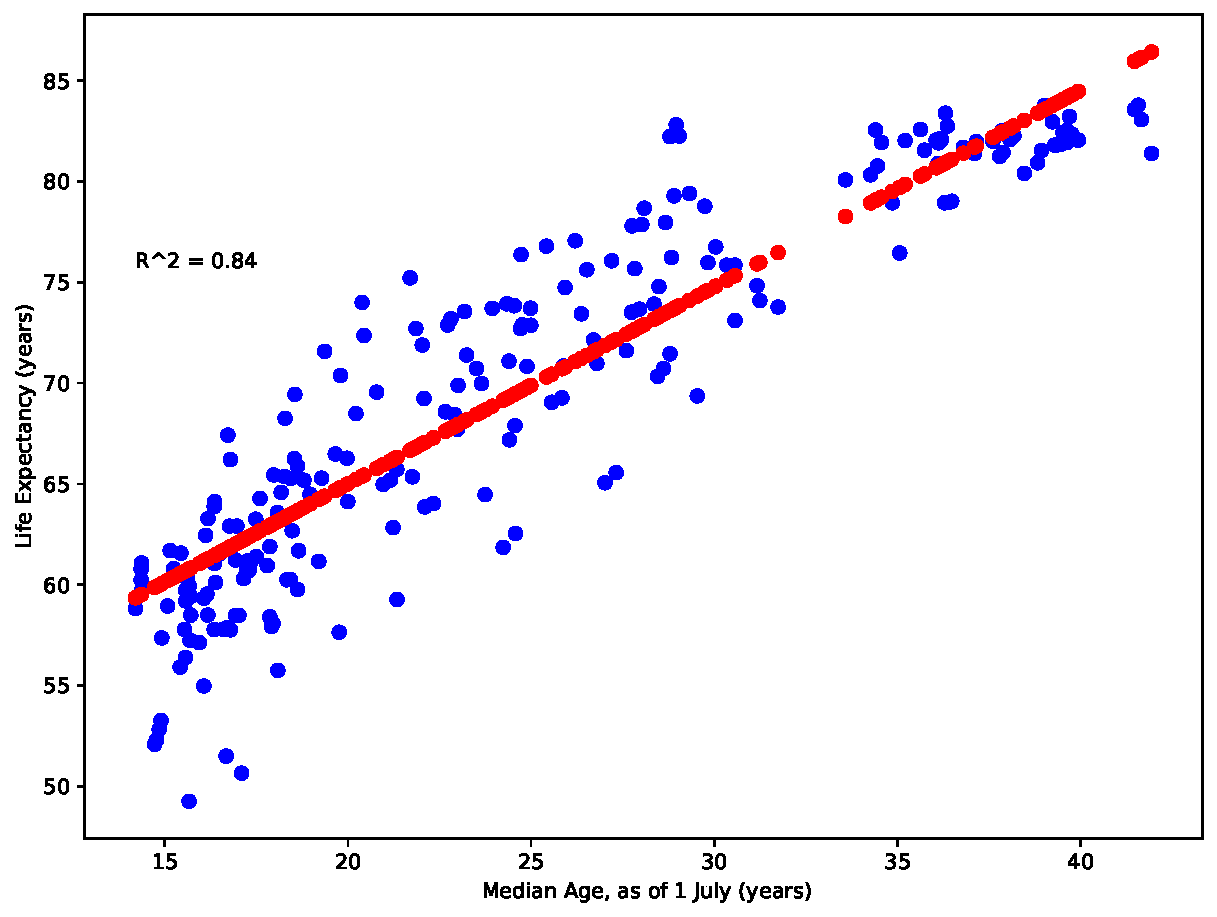
\includegraphics[width=\textwidth]{ola/_linear_regression_median_age,_as_of_1_july_(years).pdf}
      \caption{Linear Regression Median Age (original)}
      \label{fig:reg_median_age}
  \end{subfigure}
  \vfill
  \begin{subfigure}[b]{\textwidth}
      \centering
      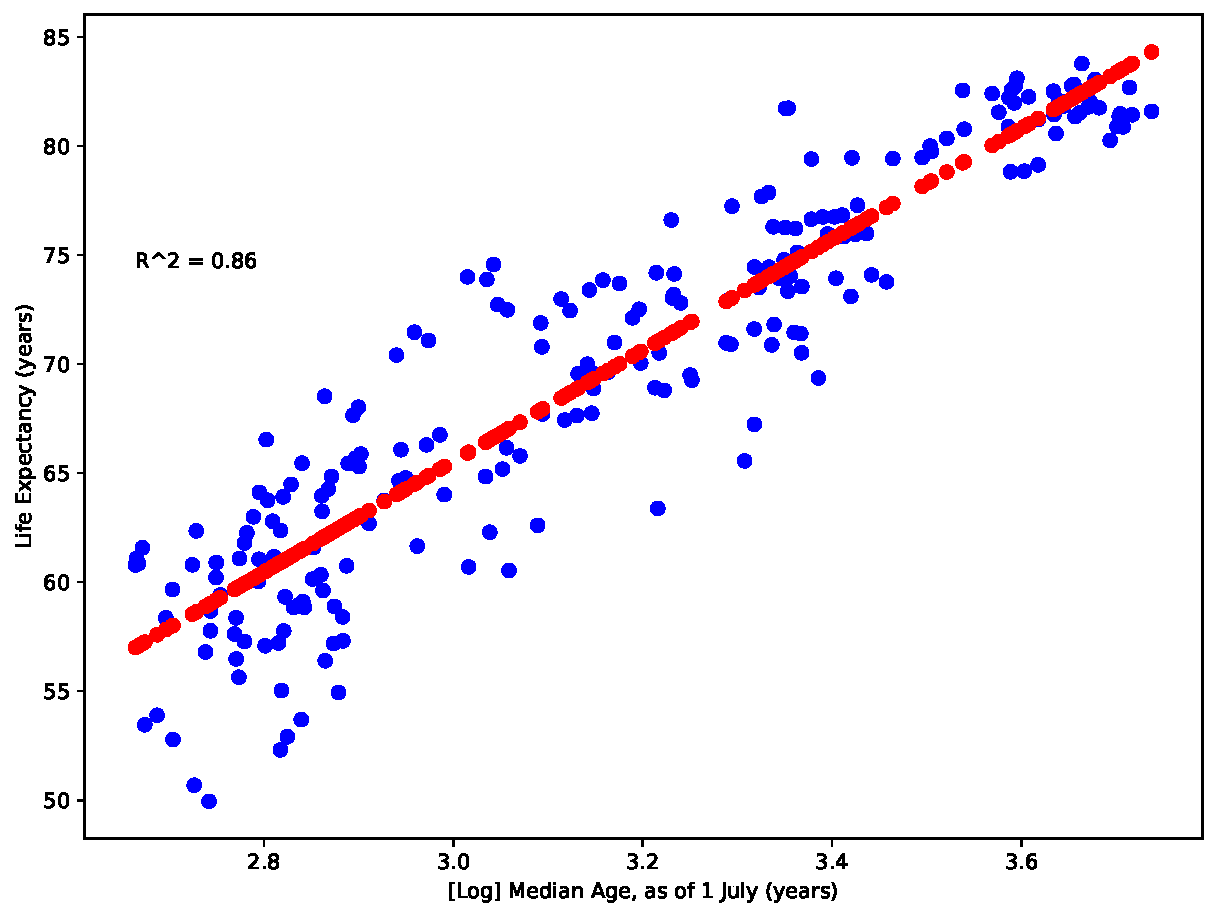
\includegraphics[width=\textwidth]{ola/[log]_linear_regression_median_age,_as_of_1_july_(years).pdf}
      \caption{Linear Regression Median Age (log)}
      \label{fig:reg_median_age_log}
  \end{subfigure}
  \caption{Linear Regression Median Age}
  \label{fig:easy_ham_and_spam_confusion_matrix}
\end{figure}

\section*{Problem 4: Mulitple linear regression}


Trained model with the following variables :  
Expected Years of Schooling, female (years), Coefficient of human inequality, Gross National Income Per Capita (2017), Median Age, as of 1 July (years), Rate of Natural Change (per 1,000 population), Crude Birth Rate (births per 1,000 population), Total Fertility Rate (live births per woman), Net Reproduction Rate (surviving daughters per woman)
The mean squared error for is 2.00.

\begin{figure}[h]
  \begin{center}
    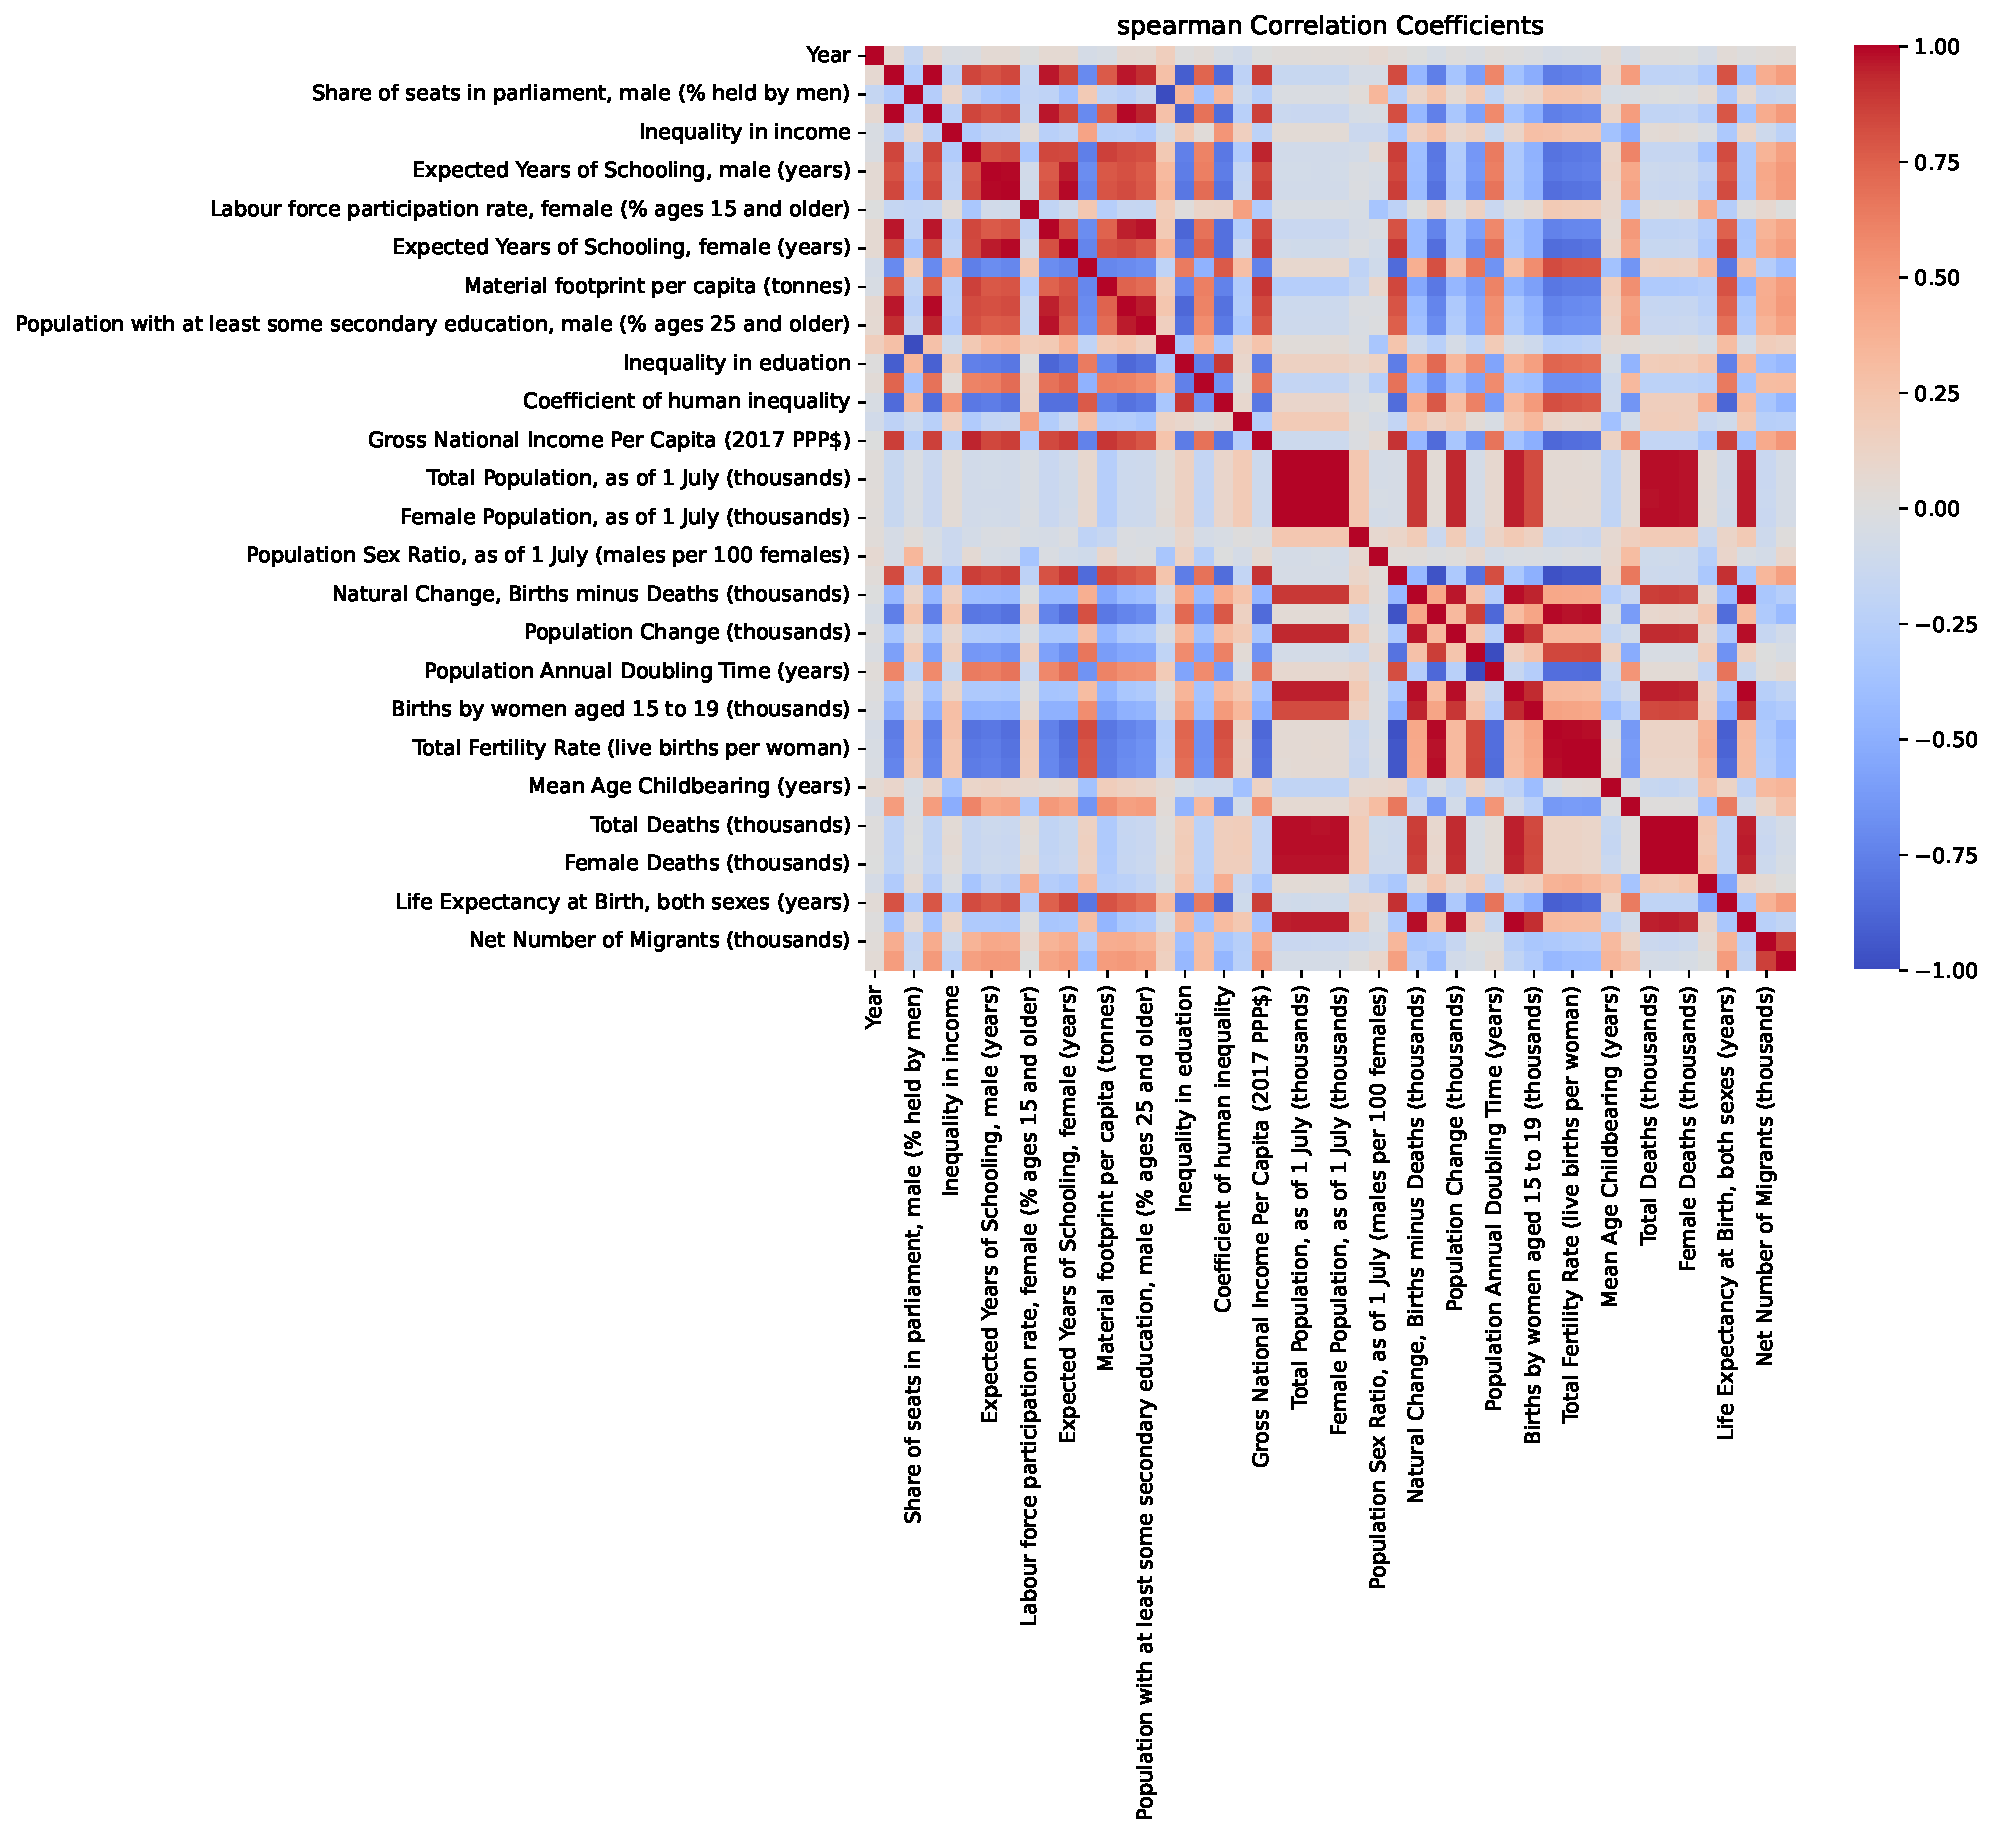
\includegraphics[width=\textwidth]{ola/spearman_correlation.pdf}
    \caption{Correlation Spearman}
    \label{fig:spearman_correlation}
  \end{center}
\end{figure}



\newpage


\printbibliography

\section*{Appendix: Source Code}

\lstset{
  language=Python,
  basicstyle=\ttfamily,
  commentstyle=\color{OliveGreen},
  keywordstyle=\bfseries\color{Magenta},
  stringstyle=\color{YellowOrange},
  numbers=left,
  basicstyle=\footnotesize,
  breaklines=true,
  postbreak=\mbox{\textcolor{red}{$\hookrightarrow$}\space}
}


\lstinputlisting{ola/assignment4.py}

\end{document}
